\chapter{Secure Hierarchical In-network Data Aggregation} % (fold)
\label{cha:Secure hierarchical In-network data aggregation}

Our work enhances Secure Hierarchical In-network data aggregation SHIA protocol of \cite{chan2006secure} by making it communication efficient, adding new capabilities to the protocol, achieving similar security goals with non-resilient aggregation functions and efficient way of analyzing the protocol.
In this chapter, we summarize the important parts of SHIA protocol and relevant terms, to build the foundation to describe our protocol in the following chapters.\\
The goal of SHIA is to compute aggregate functions (such as $\textit{truncated SUM}$, $\textit{AVERAGE}$, $\textit{COUNT}$, $\Phi-QUANTILE$) of the sensed values by the sensor nodes while assuming that partially a network is controlled by an adversary which is attempting to skew the final result.

\section{Network Assumptions}

	We assume a multi hop network with a set $ S = \{s1,...,s_{n}\} $ of $n$ sensor nodes where all $n$ nodes are alive and reachable. 
	The network is organized in a rooted tree topology.
	The trusted base station resides outside of the network and has more computation, storage capacity then the sensor nodes in the network. 
	Note that SHIA names the base station as the querier and the root of the tree as the base station. 
	The base station knows total number of sensor nodes $n$ in the network and the network topology. 
	It also has the capacity to directly communicate with every sensor node in the network.
	All the wireless communications between the nodes is peer-to-peer and we do not consider the local wireless broadcast.\\
	Each sensor node has a unique identifier $s$ and shares a unique secret symmetric key $K_{s}$ with the base station.
	The keys enable message authentication, and encryption if the data confidentiality is required.
	All the sensor nodes are capable of doing symmetric key encryption and symmetric key decryption.
	They are also capable of computing collision resistant cryptographic hash function $H$. 

\section{Attacker Model}
	
	We consider a model with a polynomially bounded adversary of \cite{przydatek2003sia}, which has a complete control over some of the sensor nodes in the network.
	Most significantly, the adversary can change the measured values reported by sensor nodes under its control.
	An adversary can perform a wide variety of attacks.
	For example, an adversary could report fictitious values (probably completely independent of the measured reported values), instead of the real aggregate values and the base station receives the fictitious aggregated information. 
	Since in many applications the information received by the base station provides a basis for critical decisions, false information could have ruinous consequences.
	However, we do not want to limit ourselves to just a few specific selected adversarial models. 
	Instead, we assume that the adversary can misbehave in any arbitrary way, and the only limitations we put on the adversary are its computational resources (polynomial in terms of the security parameter) and the fraction of nodes that it can have control over. 
	We focus on \textbf{stealthy attacks} \cite{przydatek2003sia}, where the adversary's goal is to make the base station accept false aggregation results, which are significantly different from the true results determined by the measured values, while not being detected by the base station.
	In this setting, denial-of-service (DoS) attacks such as not responding to the queries or always responding with negative acknowledgment at the end of verification phase clearly indicates to the base station that something is wrong in the network and therefore is not a stealthy attack.
	One of the security goals of the SHIA is to prevent stealthy attacks.
	
\section{Aggregate Definition and Security Goals}
	
	\begin{definition}
		According to \cite{chan2006secure}, each sensor node $s_{i}$ has a data value $a_{i}$\ assuming that all the data values are non-negative bounded by real value $a_{i} \in [0,r]$, where $r$\ is the maximum allowed data value.
		The objective of the \textbf{aggregation process} is to compute some function $f$ over all the data values, i.e., $f (a_{1}, \dotsc ,a_{n})$.
	\end{definition}

	\subsection{Security goals}
	\begin{definition}
		\label{def:direct-data-injection}
		According to \cite{chan2006secure}, a \textbf{direct data injection} attack occurs when an adversary modifies the data readings reported by the nodes under its direct control, under the constraint that only legal readings in $[0, r]$ are reported.
	\end{definition}

	Wagner \cite{wagner2004resilient} uses statistical estimation theory to quantify the effects of direct data injection on various aggregates as follows.
	An \textbf{estimator} is an algorithm $ f :\ \R^n \rightarrow \rm I\!R$\ where $f(x_{1},\dotsc, x_{n})$\ is intended as an estimate of some real valued function of $\theta$.
	We assume that $\theta$ is real valued and that we wish to estimate $\theta$ itself.
	Next, we define $\widehat{\Theta} := f(X_{1},\dotsc,X_{n})$, where $X_{1},\dotsc,X_{n}$\ are $n$ random variables. We can define the root-mean-square(r.m.s)  error (at $\theta$):
	\begin{equation}
		rms(f) := \rm I\!E[(\widehat{\Theta} - \theta)^2 | \theta]^{1/2}
	\end{equation}
	Wagner in \cite{wagner2004resilient} defines \textbf{resilient estimators and resilient aggregation } as follows.
	A $k$-node attack $A$ is an algorithm that is allowed to change up to $k$ of the values $X_{1}, \dotsc, X_{n}$ before the estimator is applied.
	In particular, the attack $A$ is specified by a function $\tau_{A} : \R^n \rightarrow  \R^n $ with the property that the vectors $x$ and $\tau_{A}(x)$ never differ at more than $k$ positions.
	We can define the root mean square(r.m.s) error associated with $A$ by
	\begin{equation}
		rms^*(f,A) := \rm I\!E[(\widehat{\Theta}^* - \theta)^2 | \theta]^{1/2} 		  
	\end{equation}
	where $\widehat{\Theta}^* := f(\tau_{A}(X_{1},\dotsc,X_{n}))$.
	To explain, $\widehat{\Theta}^*$\ is a random variable that represents the aggregate calculated at the base station in the presence of the $k$-node attack $A$, and $rms^*(f,A)$\ is a measure of inaccuracy of the aggregate after $A$'s intrusion.
	If $rms^*(f,A) >> rms(f)$, then the attack has succeeded in noticeably affecting the operation of the sensor network.
	If $rms^*(f,A) \approx rms(f)$, the attack had little or no effect.
	We define
	\begin{equation}
		rms^*(f,k) := max\{rms^*(f,A): A\ is\ a\ k-node\ attack\}
	\end{equation}
	so that $rms^*(f,k)$\ denotes the r.m.s. error of the most powerful
	$k$-node attack possible. 
	Note that $rms^* (f, 0) = rms(f)$.
	We think of an aggregation function $f$ as an instance of the resilient aggregation paradigm if $rms^* (f, k)$ grows slowly as a function of $k$.
	\begin{definition}
		According to \cite{wagner2004resilient}, an aggregation function $f$ is $(k, \alpha)$-resilient (with respect to a parameterized distribution $p(X_{i} | \theta))$ if $rms^*(f, k) \le \alpha \cdot rms(f)$ for the estimator $f$.
	\end{definition}
	The intuition is that the $(k, \alpha)$-resilient functions, for small values of $\alpha$, are the ones that can be computed meaningfully and securely in the presence of up to $k$ compromised or malicious nodes.
	\begin{table}[!htb]	
		\begin{center}
			\begin{tabular}{ |l| l| }
				\hline
			    Aggregate(f) & Security Level \\
			    \hline
			    minimum & insecure \\
			    maximum & insecure \\
			    sum & insecure \\
				average & insecure \\
				count & acceptable \\
				$[l,u]$-truncated average & problematic \\
				5\% -trimmed average & better \\
				median & much better \\
			    \hline
			\end{tabular}
		\end{center}
		 \caption{Summary of Wagner's work}
		 \label{table:wagner}
	\end{table}
	The summary of the Wagner's work is summarized in the Table~\ref{table:wagner}.
	According to this quantitative study measuring the effects of direct data injection on various aggregates, and concludes that the aggregates (truncated SUM and AVERAGE ) can be resilient under such attacks.

	Without precise knowledge of application, the direct data injection attacks are indistinguishable from the malicious sensor readings. Hence, an optimal level of aggregation security is defined as follows.  
	\begin{definition}
		\label{def:optimally-secure}
		According to \cite{chan2006secure}, an aggregation algorithm is \textbf{optimally secure} if, by tampering with the aggregation process, an adversary is unable to induce the base station to accept any aggregation result which is not already achievable by direct data injection.
	\end{definition}
	The goal of SHIA is to design an \textbf{optimally secure} aggregation algorithm with only \textbf{sublinear edge congestion}.

	\section{The SUM Aggregate Algorithm}
		In this algorithm, the aggregate function $f$\ is summation meaning that we want to compute $a_{1} + a_{2} + \dotsc + a_{n}$, where $a_{i}$\ is the sensed data value of the node $i$.
		This algorithm has three main phases:
		\begin{itemize}
			\item Query dissemination - initiates the aggregation process
			\item Aggregate commit - initiates the commitment tree generation process
			\item Result checking - initiates the distributed, interactive verification process
		\end{itemize}

	\section{Query dissemination}
		Prior to this phase, an aggregation trees is created using a tree generation algorithm.
		We can use any tree generation algorithm as this protocol works on any aggregation tree structure.
		For completeness of this protocol, one can use Tiny Aggregation Service (TaG)\cite{madden2002tag}.
		TaG uses broadcast message from the base station to initiate a tree generation.
		Each node selects its parent from whichever node it first receives the tree formation message.
		One possible aggregation tree for given network graph in Figure \ref{fig:ng} is shown in Figure \ref{fig:at}. 
		\begin{figure}[h!]
			\centering
			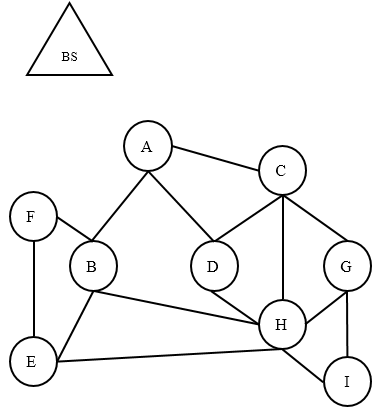
\includegraphics[scale = 1]{images/network-graph.png}\\
			\caption{Network graph}
			\label{fig:ng}
		\end{figure}
		
		To initiate the query dissemination phase, the base station broadcasts the query request message with the query nonce $N$\ in the aggregation tree. 
		The query request message contains new query nonce $N$\ for each query to prevent replay attacks in the network.
		It is very important that the same nonce is never re-used by the base station.
		$SHIA$\ uses \textbf{hash chain} to generate new nonce for each query. 
		A hash chain is constructed by repeatedly evaluating a pre-image resistant hash function $h$\ on some initial random value, the final value (or ``anchor value'') is preloaded on the nodes in the network.
		The base station uses the pre-image of the last used  value as the nonce for the next broadcast.
		For example, if the last known value of the hash chain is $h^i(X)$, then the next broadcast uses $h^{i-1}(X)$ as the nonce; $X$ is the initial random value.
		When a node receives a new nonce $N^{'}$, it verifies that $N^{'}$ is a precursor to the most recently received (and authenticated) nonce $N$ on the hash chain, i.e., $h^{i}(N^{'}) = N$ for some $i$ bounded by a fixed $k$ of number of hash applications.  
		A hash chain prevents an adversary from predicting the query nonce for future queries as it has to reverse the hash chain computation to get an acceptable pre-image.
		\begin{figure}[h!]
			\centering
			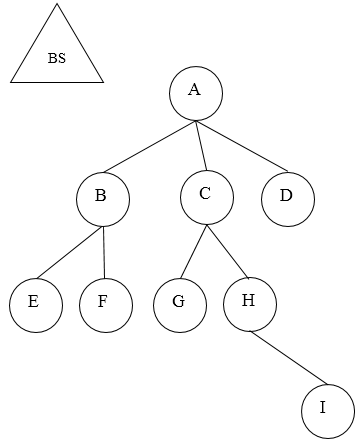
\includegraphics[scale = 1]{images/aggregation-tree.png}\\
			\caption{Aggregation tree for network graph in Figure \ref{fig:ng}}
			\label{fig:at}
		\end{figure}		
	\section{Aggregate commit} 
	% (fold)
		\label{sub:aggregate_commit}
		The aggregate commit phase constructs cryptographic commitments to the data values and to the intermediate in-network aggregation operations.
		These commitments are then passed on to the base station by the root of an aggregation tree.
		The base station then rebroadcasts the commitments to the sensor network using an authenticated broadcast so that the rest of the sensor nodes in the network can verify that their respective data values have been incorporated into the final aggregate value.

		\subsection{Aggregate commit: Naive Approach}
		% (fold)
			\label{sub:aggregate_commit_naive_approach}
			In the naive approach, during aggregation process each sensor node computes a cryptographic hash of all its inputs (including its own data value).
			The aggregation result along with the hash value called a label, is then passed on to the parent in the aggregation tree.
			The label is format is described in Definition \ref{def:label}.
			Figure \ref{fig:naive-commitment-tree} shows a commitment tree for the aggregation tree shown in Figure \ref{fig:at}.
			Conceptually, a commitment tree is a logical tree built on top of an aggregation tree, with additional aggregate information attached to the nodes to help in the result checking phase.
			\begin{figure}[h!]
				\centering
				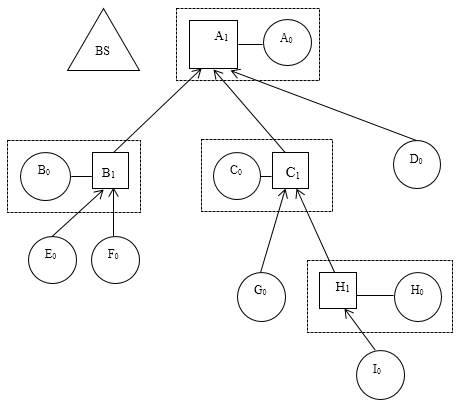
\includegraphics[scale = 1]{images/naive-commitment-tree.png}\\
				\caption{Naive commitment tree for Figure \ref{fig:at}.
				For each sensor node $s$, $s_{0}$ is its leaf vertex, while $s_{1}$ is the internal vertex representing the aggregate computation at $s$ (if any).
				The labels of the vertices on the path of node $I$ to the root are shown from Equation \ref{eq:label-1} to \ref{eq:label-5}.}
				\label{fig:naive-commitment-tree}
			\end{figure}

			\begin{definition}
				\cite{chan2006secure}
				\label{def:label}
				A commitment tree is a tree where each vertex has an associated label representing the data that is passed on to its parent. The labels have the following format:

				$\hspace{100pt}$ $<$count, value, complement, commitment$>$\\
				Where count is the number of leaf vertices in the subtree rooted at this vertex; value is the SUM aggregate computed over all the leaves in the subtree; complement is the aggregate over the COMPLEMENT of the data values; and commitment is a cryptographic commitment.
			\end{definition}
			There is one leaf vertex $u_{s}$ for each sensor node $s$, which we call the leaf vertex of $s$. The label of $u_{s}$ consists of count = 1, value = $a_{s}$ where $a_{s}$ is the data value of $s$, complement = $r - a_{s}$ where $r$ is the upper bound on allowable data values, and commitment is the node’s unique ID.\\
			Internal vertices represent aggregation operations, and have labels that are defined based on their children. Suppose an internal vertex has child vertices with the following labels: $u_{1}$, $u_{2}$, $\dotsc$ , $u_{q}$, where $u_{i}$ = $<$ $c_{i}$, $v_{i}$, $\bar{v_{i}}$,$h_{i}$$>$. 
			Then the vertex has label $<$$c$, $v$, $\bar{v}$, $h$$>$, with $c$ $=$ $\sum c_{i}$, $v$ $=$ $\sum v_{i}$, $\bar{v}$ $=$ $\sum \bar{v_{i}}$ and $h$ $=$ $H[N||c||v||\bar{v}||u_{1}||u_{2}|| \dotsc ||u_{q}]$.\\
			The labels of the vertices of the commitment tree of Figure \ref{fig:naive-commitment-tree} are shown below.
			\begin{equation}
				I_{0} = <1, a_{I}, r - a_{I}, I>
				\label{eq:label-1}
			\end{equation}
			\begin{equation}
				H_{1} = <2, v_{H_{1}}, r - v_{H_{1}}, H[N||2||v_{H_{1}}||\bar{v_{H_{1}}}||H_{0}||I_{0}]>
				\label{eq:label-2}
			\end{equation}
			\begin{equation}
				B_{1} = <3, v_{B_{1}}, r - v_{B_{1}}, H[N||3||v_{B_{1}}||\bar{v_{B_{1}}}||B_{0}||E_{0}||F_{0}]>
				\label{eq:label-3}
			\end{equation}
			\begin{equation}
				C_{1} = <4, v_{C_{1}}, r - v_{C_{1}}, H[N||4||v_{C_{1}}||\bar{v_{C_{1}}}||C_{0}||G_{0}||H_{1}]>
				\label{eq:label-4}
			\end{equation}
			\begin{equation}
				A_{1} = <9, v_{A_{1}}, r - v_{A_{1}}, H[N||9||v_{A_{1}}||\bar{v_{A_{1}}}||A_{0}||D_{0}||B_{1}||C_{1}]>
				\label{eq:label-5}
			\end{equation}
		% subsection aggregate_commit_naive_approach (end)
		
		The word vertices is used for the nodes in the commitment tree and the word node is used for the nodes in the aggregation tree.
		There is a mapping between the nodes in the aggregation tree and the vertices in the commitment tree, a vertex is a logical element in the commitment tree where as the node is a physical sensor node which does all the communications.		
		The collision resistant hash function makes it impossible for an adversary to change the commitment structure once it is sent to the base station.
		Our payload format is compact than the label format which is discussed in the next chapter.
		
		\subsection{Aggregate commit: Improved approach} 
		% (fold)
			\label{sub:aggregate_commit_improved_approach}
			The aggregation tree is a subgraph of the network graph so it may be randomly unbalanced.
			This approach tries to separate the structure of the commitment tree from the structure of the aggregation tree.
			So, the commitment tree can be perfectly balanced.

			In the naive approach, each sensor node always computes the aggregate sum of all its inputs which is a greedy approach.
			SHIA uses delayed aggregation approach, which performs an aggregation operation if and only if it results in a complete, binary commitment tree.

			We now describe SHIA's delayed aggregation algorithm for producing balanced commitment trees.
			In the naive commitment tree, each sensor node passes to its parent a single message containing the label of the root vertex of its commitment subtree $T_{s}$.
			In the delayed aggregation algorithm, each sensor node passes on the labels of the root vertices of a set of commitment subtrees $F = \{ T_{1}, \dotsc, T_{q} \}$.
			We call this set a commitment forest, and we enforce the condition that the trees in the forest must be complete binary trees, and no two trees have the same height. 
			These constraints are enforced by continually combining equal-height trees into complete binary trees of greater height.
			\begin{definition}
				\cite{chan2006secure}
				\label{def:commitment-forest}
				A commitment forest is a set of complete binary commitment trees such that there is at most one commitment tree of any given height.
			\end{definition}

			The commitment forest is built as follows. Leaf sensor nodes in the aggregation tree originate a single-vertex commitment forest, which they then communicate to their parent sensor nodes. Each internal sensor node $s$ originates a similar single-vertex commitment forest.
			In addition, $s$ also receives commitment forests from each of its children.
			Sensor node $s$ keeps track of which root vertices were received from which of its children.
			It then combines all the forests to form a new forest as follows.
			Suppose $s$ wishes to combine $q$ commitment forests $F_{1}$,$\dotsc$,$F_{q}$.
			Note that since all commitment trees are complete binary trees, tree heights can be determined by inspecting the count field of the	root vertex.
			We let the intermediate result be $F$ $=$ $F_{1}$ $\cup$ $\dotsc$ $\cup$ $F_{q}$, and repeat the following until no two trees are the same height in $F$.
			Let $h$ be the smallest height such that more than one tree in $F$ has height $h$.
			Find two commitment trees $T_{1}$ and $T_{2}$ of height $h$ in $F$, and merge them into a tree of height $h + 1$ by creating a new vertex that is the parent of both the roots of $T_{1}$ and $T_{2}$ according to the inductive rule in Definition \ref{def:label}.

			\begin{exmp} The commitment-forest generation process for node $A$ of Figure \ref{fig:at} is shown here.\\
				\begin{figure}[h!]
					\centering
					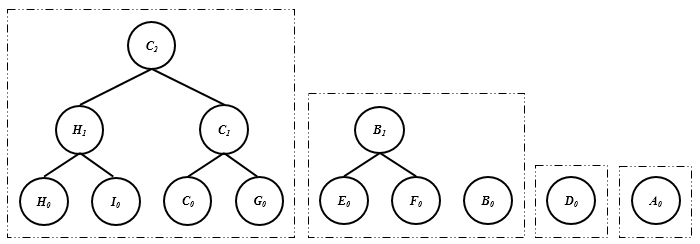
\includegraphics[scale = 0.9]{images/commitment-tree-example-1-shia.png}\\
					\caption{$A$ receives $C_{2}$ from $C$, $(B_{1},B_{0})$ from $B$, $D_{0}$ from $D$ and generates $A_{0}$. The commitment forest received from a given sensor node is indicated by dashed-line box.}
					\label{fig:commitment-tree-example-1-shia}
				\end{figure}\\

				\begin{equation}
					\begin{array}{l}
						A_{0} = <1, a_{A}, r - a_{A}, A>\\
						D_{0} = <1, a_{D}, r - a_{D}, D>\\
						E_{0} = <1, a_{E}, r - a_{E}, E>\\
						B_{1} = <2, v_{B_{1}}, \bar{v_{B_{1}}}, H(N || 2 || v_{B_{1}}|| \bar{v_{B_{1}}} || B_{0} || F_{0})>\\
						C_{2} = <4, v_{C_{2}}, \bar{v_{C_{2}}}, H(N || 4 || v_{C_{2}}|| \bar{v_{C_{2}}} || H_{1} || C_{1})>\\
					\end{array}
				\end{equation}
				\begin{figure}[h!]
					\centering
					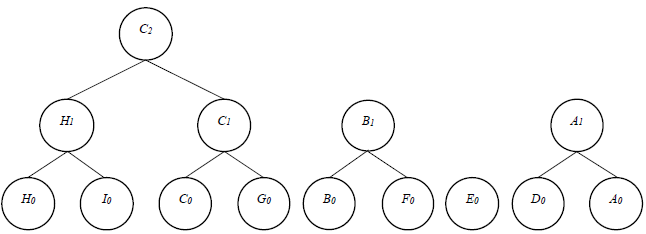
\includegraphics[scale = 1]{images/commitment-tree-example-2-shia.png}\\
					\caption{First Merge: $A_{1}$ vertex created by A.}
					\label{fig:commitment-tree-example-2-shia}
				\end{figure}
				\begin{equation}
					\begin{array}{l}
						A_{1} = <2, v_{A_{1}}, \bar{v_{A_{1}}}, H(N || 2 || v_{A_{1}}|| \bar{v_{A_{1}}} || A_{0} || D_{0})>\\
						v_{A_{1}} = a_{A} + a_{D}; \bar{v_{A_{1}}} = r - a_{A} + r - a_{D}\\
					\end{array}
				\end{equation}
				\begin{figure}[h!]
					\centering
					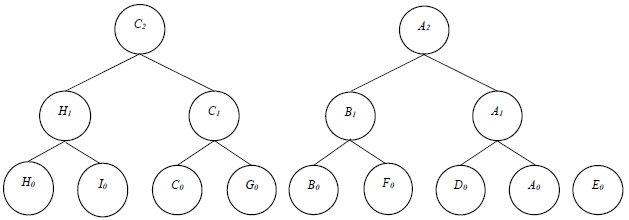
\includegraphics[scale = 1]{images/commitment-tree-example-3-shia.png}\\
					\caption{Second Merge: $A_{2}$ vertex created by A.}
					\label{fig:commitment-tree-example-3-shia}
				\end{figure}
				\begin{equation}
					\begin{array}{l}
						A_{2} = <4, v_{A_{2}},\bar{v_{A_{2}}},H(N || 4 || v_{A_{2}} || \bar{v_{A_{2}}} || B_{1} ||A_{1}) >\\
						v_{A_{2}} = v_{A_{1}} + v_{B_{1}}; \bar{v_{A_{2}}} = r - v_{A_{1}} + r - v_{B_{1}}
					\end{array}
				\end{equation}
				\begin{figure}[h!]
					\centering
					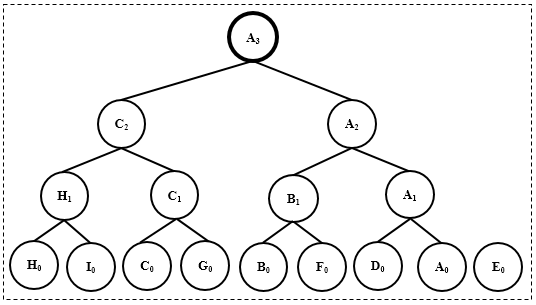
\includegraphics[scale = 1]{images/commitment-tree-example-4-shia.png}\\
					\caption{Third Merge: $A_{3}$ vertex created by A.}
					\label{fig:commitment-tree-example-4-shia}
				\end{figure}
				\begin{equation}
					\begin{array}{l}
						A_{3} = <8, v_{A_{3}},\bar{v_{A_{3}}},H(N || 8 || v_{A_{3}} || \bar{v_{A_{3}}} || C_{2} ||A_{2}) >\\
						v_{A_{3}} = v_{A_{2}} + v_{C_{2}}; \bar{v_{A_{3}}} = r - v_{A_{2}} + r - v_{C_{2}}
					\end{array}
				\end{equation}
			\end{exmp}
		% subsection aggregate_commit_improved_approach (end)
	% section aggregate_commit (end)

\section{Result checking} % (fold)
\label{sec:result_checking}
	SHIA presents novel distributed verification algorithm achieving provably optimal security while maintaining sublinear edge congestion.
	In our work, we take similar approach and add new capabilities to help find an adversary.
	Here, we describe the SHIA's result checking phase to build the basis for our work.
	The purpose of the result checking phase is to enable each sensor node $s$ to independently verify that its data value as was added into the SUM aggregate, and the complement $(r - a_{s})$ of its data value was added into the COMPLEMENT aggregate. 
	First, the aggregation results from the aggregation-commit phase are sent by the base station using authenticated broadcast to every sensor node in the network.
	Each sensor node then individually verifies that its contributions to the respective SUM and COMPLEMENT aggregates were indeed counted.
	If so, it sends an authentication code to the base station.
	The authentication code is also aggregated for communication efficiency. 
	When the base station has received all the authentication codes, it is then able to verify that all sensor nodes have checked that their contribution to the aggregate has been correctly counted.
	The result checking process has the following phases.\\
	\textbf{Dissemination of final commitment values.}
	Once the base station receives final commitment labels from the root of the commitment forest, it sends each of those commitment labels to the entire network using authenticated broadcast.
	Authenticated broadcast means that the each sensor node can verify that the message was sent by the base station and no one else.\\
	\textbf{Dissemination of off-path values.} 
	Each vertex must receive all of its off-path values to do the verification.
	The off-path values are defined as follows.
	\begin{definition}
		\cite{chan2006secure}
		The set of off-path vertices for a vertex $u$ in a tree is the set of all the siblings of each of the vertices on the path from $u$ to the root of the tree that $u$ is in (the path is inclusive of $u$).
	\end{definition}
	\begin{figure}[h!]
		\centering
		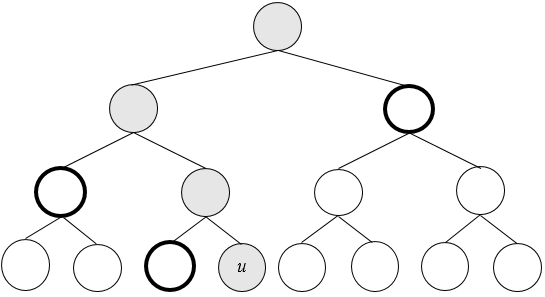
\includegraphics[scale = 1]{images/off-path.png}\\
		\caption{Off-path vertices from $u$ are highlighted in bold.}
		\label{fig:commitment-tree-example-2-shia}
	\end{figure}
	Vertex receives its off-path values from its parent.
	Each internal vertex has two children.
	For example, an internal vertex $k$\ has two children $k_{1},k_{2}$.
	$k$\ sends the label of $k_{1}$\ to $k_{2}$\ and vice versa.
	$k$\ tags the relevant information of its left and right child.
	Once a vertex receives all of its off-path values it begins a verification phase.
	\textbf{Verification of contribution.}
	The leaf vertex calculates the root vertex's label using its own label and off-path vertex labels.
	This allows the leaf to verify that its label was not modified on the path to the root during the aggregation-commit process. 
	Then it compares the the calculated root vertex's label with the label received from the base station via authenticated broadcast.
	If those two labels match then it proceeds to the next step with ACK message or with NACK message.\\
	\textbf{Collection of authentication codes.} Once each sensor node $s$\ does verification of contribution for its leaf vertex $v_{s}$\ it sends the relevant authentication code to the base station.
	The authentication code for sensor node $s$\ with ACK and NACK message has the following format.
	\begin{equation}
		MAC_{K_{s}}(N||ACK)	
	\end{equation}
	\begin{equation}
		MAC_{K_{s}}(N||NACK)	
	\end{equation}
	Where ACK, NACK are unique message identifier for positive acknowledgment and negative acknowledgment respectively, $N$ is the query nonce and $K_{s}$\ is secret key that $s$\ shares with the base station.
	Collection of authentication code starts with the leaf nodes in the aggregation tree.
	Leaf nodes in the aggregation tree send their authentication codes to their parent.
	Once the parent node has received the authentication from all of its children it does XOR operation on all the authentication codes including its own authentication code and sends it to its parent in the aggregation tree.
	Each internal sensor node $s$\ in the aggregation tree repeats the process.
	Finally, the root of an aggregation tree sends a single authentication code to the base station which is an XOR of all the authentication codes of the aggregation tree.\\  
	\textbf{Verification of confirmations.}
	Since the base station knows the key $K_{s}$ for each sensor node $s$, it verifies that every sensor node has released its authentication code by computing the XOR of the authentication codes for all the sensor nodes in the network, i.e., $\bigoplus_{i = 1}^n MAC_{K_{i}}(N || ACK)$.
	The base station then compares the computed code with the received code. If the two codes match, then the base station accepts the aggregation result.

	\begin{theorem}
		\cite{chan2006secure}
		Let the final SUM aggregate received by the base station be $S$.
		If the base station accepts $S$, then $S_{L} \leq S \leq (SL + \mu \cdot r)$ where $S_{L}$ is the sum of the data values of all the legitimate nodes, $\mu$ is the total number of malicious nodes, and $r$ is the upper bound on the range of allowable values on each node.
	\end{theorem}
	The above theorem is proven by SHIA. SHIA achieves security over the truncated SUM which is a resilient aggregator according to Wagner\cite{wagner2004resilient}.
	Our protocol works on SUM which is non-resilient aggregate and achieves the similar security goals. 
% section result_checking (end)